\documentclass{article}

\usepackage{graphicx}
\usepackage{tikz}
\usepackage{tikzsymbols}
\usetikzlibrary{calc,patterns,shapes.geometric}
\pagestyle{empty}
\usepackage[margin=0pt]{geometry}
\geometry{papersize={14in,12in}}

\def\centerarc[#1](#2)(#3:#4:#5){\draw[#1] ($(#2)+({#5*cos(#3)},{#5*sin(#3)})$) arc (#3:#4:#5);}

\begin{document}
	\begin{figure}
		\centering
		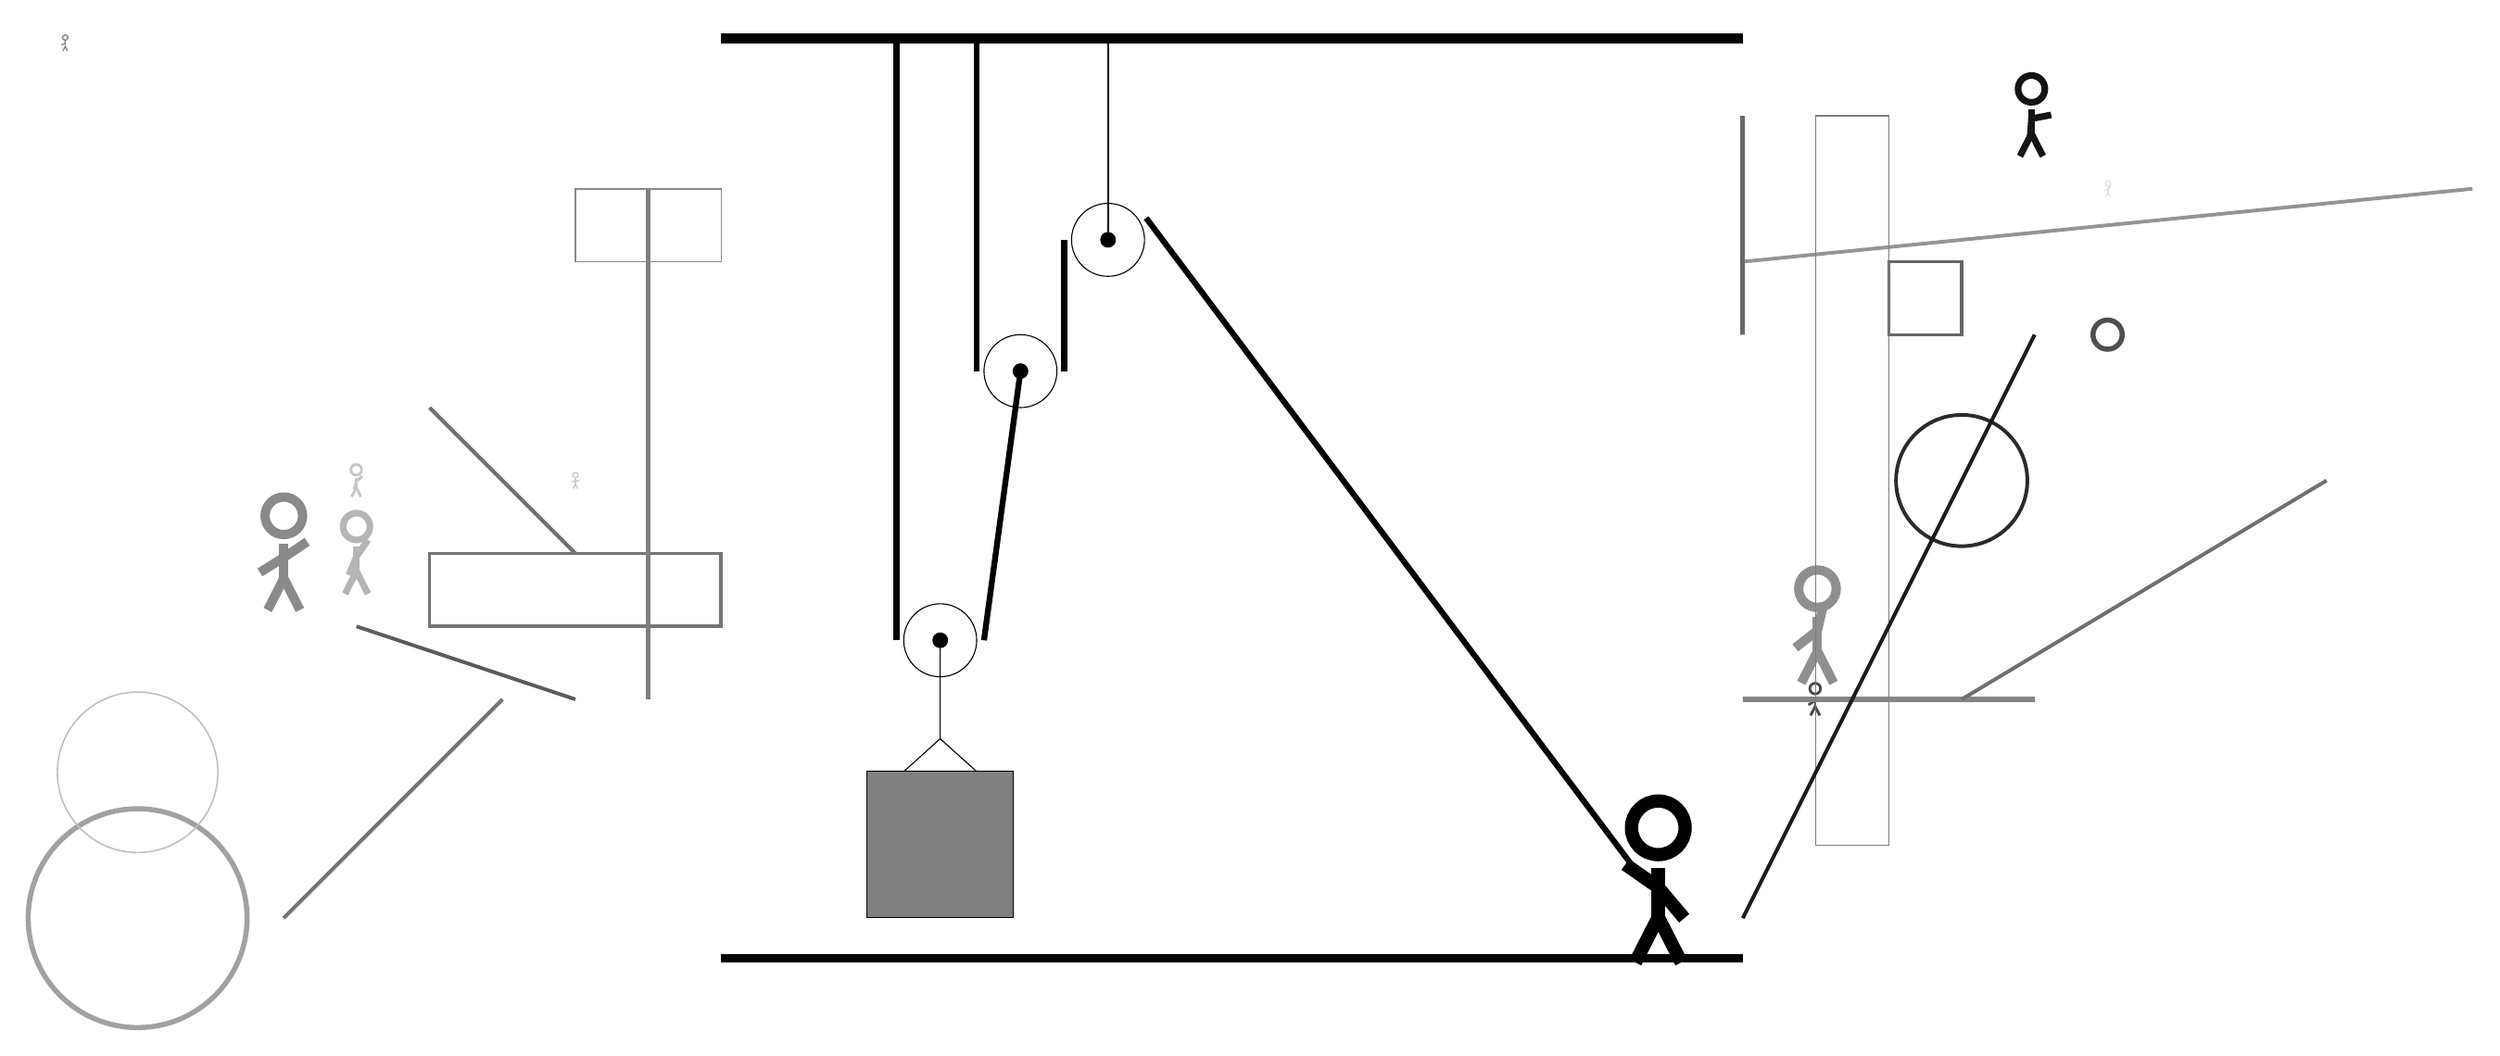
\begin{tikzpicture}
			%%%%% START %%%%%
			
			\draw[fill=black] (-2, 9) rectangle (12, 9.125);
			
			\draw (1, 0.81) circle (0.5);
			\draw[fill=black] (1, 0.81) circle (0.1);
			
			\draw (2.1, 4.5) circle (0.5);
			\draw[fill=black] (2.1, 4.5) circle (0.1);
			
			\draw (3.3, 6.3) circle (0.5);
			\draw[fill=black] (3.3, 6.3) circle (0.1);
			\draw[thick] (3.3, 6.3) -- (3.3, 9);
			
			\draw [line width=0.5mm, color=black!83](15, 3) circle (0.9);
			
			\draw[line width=0.5mm, color=black!57](-4, 2) -- (-6, 4);
			\draw[line width=0.5mm, color=black!42](12, 6) -- (22, 7);
			\draw[line width=0.5mm, color=black!54](-5, 0) -- (-8, -3);
			\node[line width=0.3mm, color=black!29] at (-7, 2) {\Strichmaxerl[5][68][55]};
			\node[line width=0.7mm, color=black!71] at (13, 0) {\Strichmaxerl[2][33][11]};
			\draw [line width=0.7mm, color=black!69](17, 5) circle (0.2);
			
			\node[line width=0.3mm, color=black!22] at (-7, 3) {\Strichmaxerl[2][74][43]};
			\draw[line width=0.5mm, color=black!54] (-2, 1) rectangle (-6, 2);
			\draw[line width=0.6mm, color=black!50] (-3, 0) rectangle (-3, 7);
			\node[line width=0.3mm, color=black!21] at (-4, 3) {\Strichmaxerl[1][8][5]};
			\draw[line width=0.7mm, color=black!48] (12, 0) rectangle (16, 0);
			\draw[line width=0.5mm, color=black!56](15, 0) -- (20, 3);
			
			\draw [line width=0.7mm, color=black!37](-10, -3) circle (1.5);
			\draw[line width=0.2mm, color=black!46] (-4, 6) rectangle (-2, 7);
			\node[line width=0.6mm, color=black!44] at (13, 1) {\Strichmaxerl[7][38][77]};
			
			\draw[line width=0.4mm, color=black!60] (14, 6) rectangle (15, 5);
			\draw [line width=0.2mm, color=black!25](-10, -1) circle (1.1);
			\draw[line width=0.6mm, color=black!59] (12, 5) rectangle (12, 8);
			\node[line width=0.5mm, color=black!12] at (17, 7) {\Strichmaxerl[1][22][55]};
			\node[line width=0.4mm, color=black!46] at (-11, 9) {\Strichmaxerl[1][19][89]};
			\draw[line width=0.2mm, color=black!51] (14, -2) rectangle (13, 8);
			\draw [line width=0.3mm, color=black!81](-5, -2) circle (0.0);
			\node[line width=0.2mm, color=black!92] at (16, 8) {\Strichmaxerl[5][86][11]};
			\node[line width=0.2mm, color=black!46] at (-8, 2) {\Strichmaxerl[7][32][34]};
			
			\draw[line width=0.5mm, color=black!64](-4, 0) -- (-7, 1);
			\draw[line width=0.5mm, color=black!89](12, -3) -- (16, 5);
			
			\draw (1, 0.81) -- (1, -0.54) -- (0.5, -0.99) -- (1.5, -0.99) -- (1, -0.54);
			\draw[fill=black!50] (0, -0.99) rectangle (2, -2.99);
			
			\draw[line width=0.8mm] (0.4, 9) -- (0.4, 0.81);
			\centerarc[line width=0.8mm](1, 0.81)(180:360:0.6);
			\draw[line width=0.8mm](1.6, 0.81) -- (2.1, 4.5);
			\draw[line width=0.8mm] (1.5, 9) -- (1.5, 4.5);
			\centerarc[line width=0.8mm](2.1, 4.5)(180:360:0.6);
			\draw[line width=0.8mm](2.7, 4.5) -- (2.7, 6.3);
			\centerarc[line width=0.8mm](3.3, 6.3)(30:180:0.6);
			\draw[line width=0.8mm] (3.822, 6.6) -- (10.5, -2.3);
			
			\node at (10.8, -2.5) {\Strichmaxerl[10][-35][-50]};
			
			\draw[fill=black] (-2, -3.5) rectangle (12, -3.6);
			
			%%%%% END %%%%%
		\end{tikzpicture}
	\end{figure}	
\end{document}